\section{Numerical Analysis}

In this section, we numerically evaluate the proposed noise inference procedure on two representative examples. The first is a small, arbitrary graph that serves as a transparent validation of the proposed method. The second is a 2D cluster-state, used to assess the estimator's performance on a larger, more structured graph. Throughout this section, we work with an effective one-parameter per edge description, and denote by $\lambda_{e}$ the effective noise parameter associated with edge $e\in E$. This edge-level description is the effective parametrization used for the numerical reconstruction in this section, and serves as a compressed version of the more detailed notation introduced in Section~\ref{sec:Depnoise}. For a given gate ordering $C$ and trap qubit $v$, the corresponding trap bias is modeled as
\begin{equation}
	P_v(C)=\prod_{e\in S_v(C)} \lambda_e,
\end{equation}
where $S_v(C)$ is the set of edges whose propagated Pauli contributions affect the trap outcome at $v$ under ordering $C$. In the numerical simulations, the trap-failure probabilities are estimated from finite samples, and the corresponding empirical trap biases are used to reconstruct the parameters $\lambda_{e}$. The main purpose of this section is twofold. First, we verify that the ordering-based ratio estimator correctly isolates the contribution of individual edges. Second, we study how the reconstruction accuracy improves with the number of measurement samples.

\subsection{Arbitrary graph example}

We first consider the graph shown in ~\cref{fig:diamond-kite-direct-alternate}, with vertex set $V=\{1,2,3,4\}$ and edge set $E=\{(1,2),(1,4),(2,3),(2,4),(3,4)\}$. The corresponding unknown effective noise parameters are $\lambda_{(1,2)},\ \lambda_{(1,4)},\ \lambda_{(2,3)},\ \lambda_{(2,4)},\ \lambda_{(3,4)}$.


\begin{figure}[H]
  \centering
  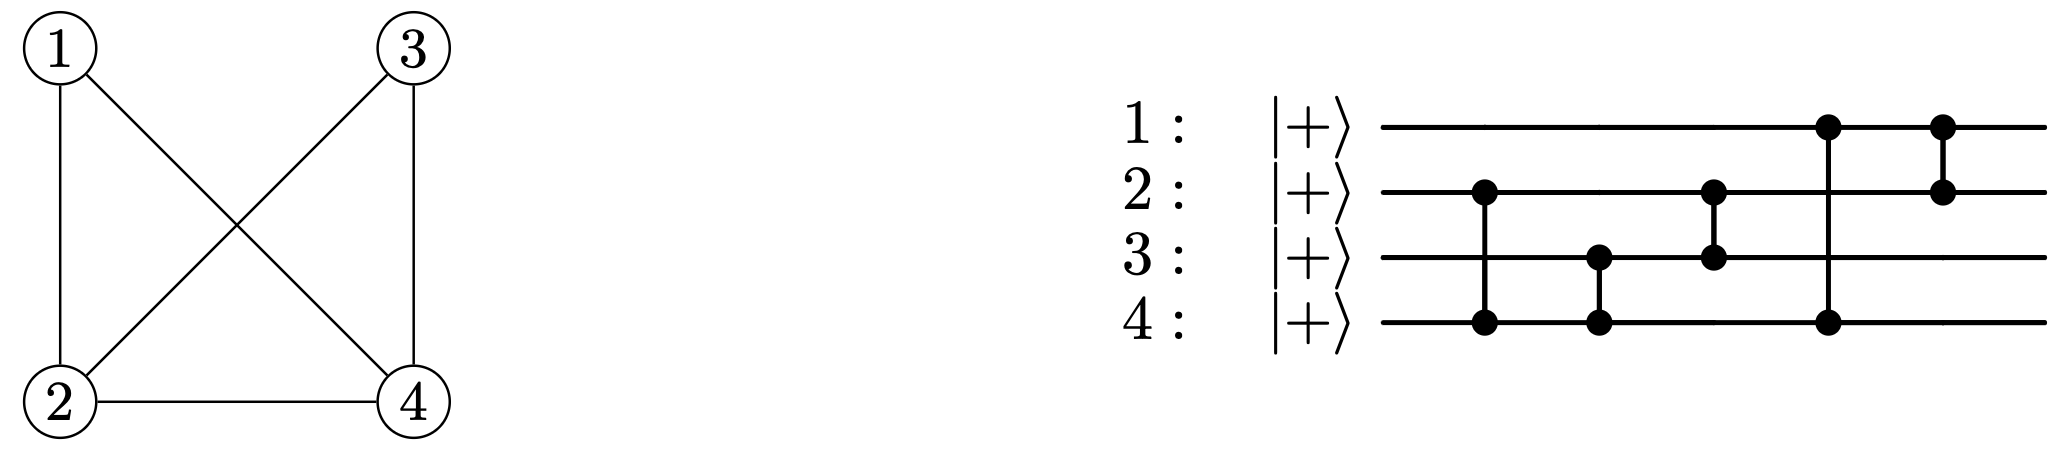
\includegraphics[scale=0.35]{arbitrary.png}
  \caption{Graph state with edges \(E=\{(2,4),(2,3),(3,4),(1,4),(1,2)\)\} and all qubits initialized in \(\ket +\)}
  \label{fig:diamond-kite-direct-alternate}
\end{figure}


For this example, we use a homogeneous one-qubit depolarizing noise model in order to make the reconstruction mechanism fully explicit. After each $\mathrm{CZ}$ gate, each involved qubit is subjected to a depolarizing channel with error probability $p_{\mathrm{err}}=0.002$. The associated effective parameter is then
$\lambda_{\mathrm{th}}=1-\frac{4}{3}p_{\mathrm{err}}=1-\frac{4}{3}(0.002)=0.997333\ldots$. Under this uniform setting, all edge parameters take the same value, $\lambda_{(1,2)}=\lambda_{(1,4)}=\lambda_{(2,3)}=\lambda_{(2,4)}=\lambda_{(3,4)}=\lambda_{\mathrm{th}}$.


We now illustrate how one of these parameters can be recovered from trap statistics. Consider the trap associated with qubit $1$, corresponding to the stabilizer generator $K_1=X_1\otimes Z_2\otimes Z_4$. For a reference ordering $C$, suppose that the propagated support contributing to the trap bias at qubit $1$ is $S_1(C)=\{(1,2),(1,4),(2,3),(2,4),(3,4)\}$, then $P_1(C)= \lambda_{(1,2)}\lambda_{(1,4)}\lambda_{(2,3)}\lambda_{(2,4)}\lambda_{(3,4)} \approx 0.9867376$.

Next, we choose another ordering $C'$ such that the contribution of edge $(2,3)$ is removed while all other contributions remain unchanged, namely $S_1(C')=S_1(C)\setminus\{(2,3)\}$. This gives
$P_1(C')=\lambda_{(1,2)}\lambda_{(1,4)}\lambda_{(2,4)}\lambda_{(3,4)}\approx 0.9893759$.
Taking the ratio of the two trap biases isolates the parameter of the missing edge:
\begin{equation}
	\widehat{\lambda}_{(2,3)}
	=
	\frac{P_1(C)}{P_1(C')}
	\approx
	\frac{0.9867376}{0.9893759}
	\approx 0.997333,
\end{equation}
which agrees with the theoretical value $\lambda_{\mathrm{th}}$.

The same procedure can be repeated for the other edges by selecting suitable trap qubits and pairs of orderings. This example, therefore, serves as a numerical validation of the estimator, i.e., the effective edge parameter is recovered directly from simulated trap statistics, and the reconstructed value matches the injected noise parameter.

\subsection{2D cluster-state example}

We now consider a 2D cluster-state with vertices arranged on a $W \times H$ square lattice as described in \cref{fig:2d-cluster} and edges connecting nearest neighbours horizontally and vertically. In this case, the graph is significantly larger, and the numerical study is used to assess the behavior of the reconstruction method under heterogeneous noise and finite sampling. As in the previous sections, multiple global orderings of the commuting $\mathrm{CZ}$ gates are generated from the ordered-triple construction and the associated conflict graph. These orderings are then used to produce distinct trap-bias equations from which the effective edge parameters are reconstructed.

In contrast to the arbitrary-graph example, the noise is now non-uniform. Specifically, after each $\mathrm{CZ}$ gate, the one-qubit depolarizing error probability acting on each involved qubit is sampled independently from a Gaussian distribution, 
\begin{equation}\label{equ:gaus}
p \sim \mathcal{N}\!\left(10^{-2},\,2\times 10^{-3}\right), \mathcal{N}\!\left(10^{-2},\,2\times 10^{-4}\right), \dots, \mathcal{N}\!\left(10^{-2},\,2\times 10^{-7}\right).
\end{equation}
In the numerical implementation, the sample values are truncated to the physical interval $[0,1]$ whenever necessary. For each sampled value of $p$, the corresponding one-qubit depolarizing factor is computed as $\lambda = 1-\frac{4}{3}p$.

Thus, the simulation is generated from the underlying qubit after gate noise samples rather than from a single uniform noise parameter. The quantities $\lambda_{e}$ appearing in the reconstruction are therefore effective edge-level parameters inferred from the resulting trap-bias equations. For a given ordering $C$ and trap qubit $v$, the trap-failure probability is estimated from the sampled outcomes as
\begin{equation}
	\widehat{p}_{\mathrm{fail}}(v,C)
	=
	\frac{N_{\mathrm{fail}}(v,C)}{N_{\mathrm{shots}}(v,C)},
\end{equation}
and the corresponding empirical trap bias is $\widehat{P}_v(C)=1-2\widehat{p}_{\mathrm{fail}}(v,C)$.
Using the family of generated orderings, these empirical trap biases produce an overdetermined system for the unknown parameters $\lambda_{e}$, whose solution yields the reconstructed values $\widehat{\lambda}_e$.










For the numerical study, we take a cluster-state of width $W=12$ and depth $H=12$.
Reconstruction quality is evaluated from the distributions of the signed differences
$\widehat{\lambda}_e-\lambda_e$ and the absolute deviations
$100\times |\widehat{\lambda}_e-\lambda_e|$ over all reconstructed edges.
For each of the five Gaussian noise spreads in Eq.~\eqref{equ:gaus}, we compare
three shot budgets: $10^4$, $10^5$, and $10^6$. Figs.~\ref{fig:lambda_diff_by_shots}~$-$~\ref{fig:lambda_abs_diff_by_shots} report the corresponding
histograms. 



Several features are consistent across all five noise ensembles. First, the histograms of
$\widehat{\lambda}_e-\lambda_e$ remain centered close to zero, indicating that the estimator
does not exhibit a visible systematic bias. Second, the distributions narrow markedly as the
number of shots increases from $10^4$ to $10^6$, which is the expected finite-sampling
behavior. The same trend is visible in the histograms of the absolute deviations, whose mass
becomes progressively more concentrated near zero as the shot count increases. This shows that
the reconstructed parameters become more stable and more accurate when more trap rounds are
available. 

A second trend appears when comparing Figs.~\ref{fig:lambda_diff_by_shots}~$-$~\ref{fig:lambda_abs_diff_by_shots} with one another. As the variance of the
underlying Gaussian sampling is reduced from $2\times 10^{-3}$ to $2\times 10^{-7}$, the
reconstructed distributions become increasingly concentrated. This is consistent with the fact
that smaller spread in the injected qubit-level noise yields a more homogeneous effective
edge-level model, which is easier to reconstruct from the available trap statistics. Taken
together, these results support the effectiveness of the proposed inference method on a large
and structured graph. In other words, the ordering-based reconstruction remains stable under heterogeneous
noise and improves predictably with increasing sample size.


\begin{figure}[!h]
	\centering
    \begin{subfigure}{0.48\textwidth}
    %%\centering
	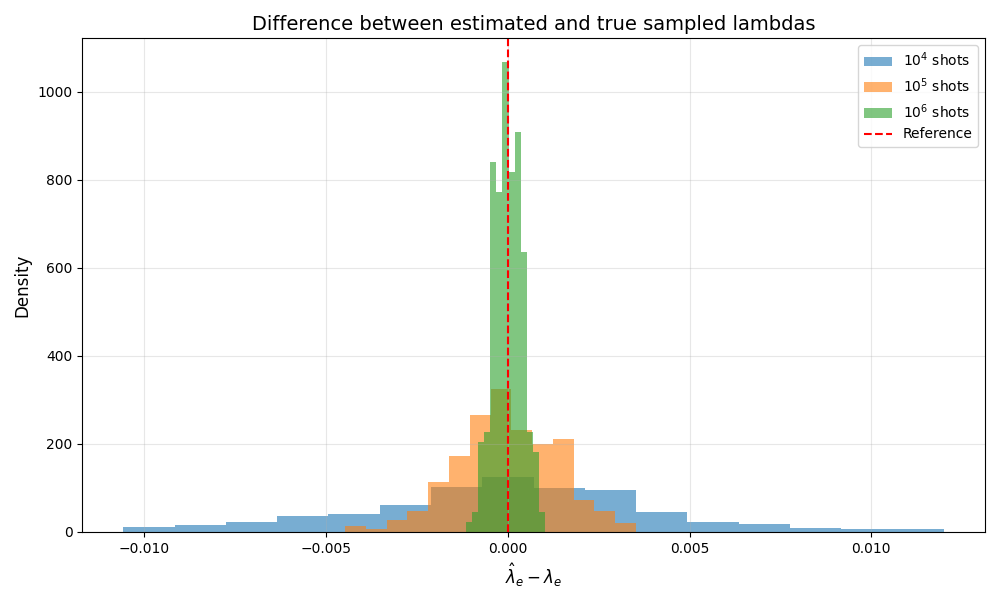
\includegraphics[width=\linewidth]{plot_lambda_diff_by_shots_sd.png}
    %\caption{}
	%\caption{Distribution of the reconstruction differences for the 2D cluster-state with $12 \times 12$ simulation, shown for $10^4$, $10^5$, and $10^6$ shots. The dashed red line indicates zero difference. The distribution becomes increasingly concentrated around zero as the number of shots increases.}
	%\label{fig:lambda_diff_by_shots}
    \end{subfigure}
\hfill
\begin{subfigure}{0.48\textwidth}
	%\centering
	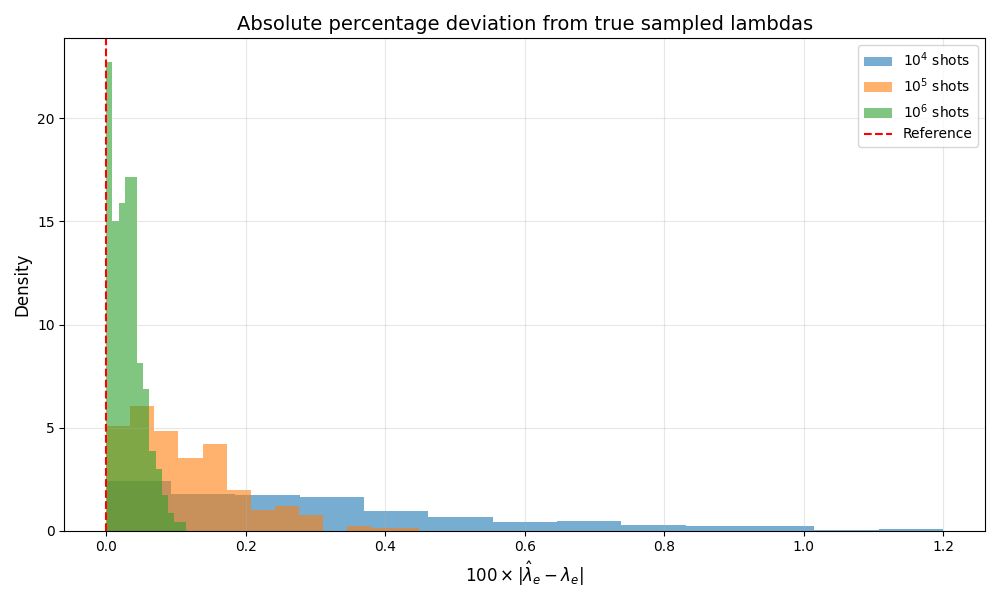
\includegraphics[width=\linewidth]{plot_lambda_diff_abs_by_shots_sd.png}
    %\caption{}
	%\caption{Distribution of the absolute reconstruction deviations for the 2D cluster-state with $12 \times 12$ simulation, shown for $10^4$, $10^5$, and $10^6$ shots. The improved concentration near zero with increasing shot count indicates better reconstruction accuracy.}
	%\label{fig:lambda_abs_diff_by_shots}
\end{subfigure}
%%\vspace{-0.4cm}
\caption{Distribution of the reconstruction differences $\widehat{\lambda}_e-\lambda_e$
(left) and of the absolute deviations $100\times |\widehat{\lambda}_e-\lambda_e|$ (right)
for the $12\times 12$ 2D cluster-state, using $10^4$, $10^5$, and $10^6$ shots, when the
post-$\CZ$ one-qubit depolarizing error probabilities are sampled independently from
$\mathcal{N}(10^{-2},\,2\times 10^{-3})$. The dashed red line marks zero difference. As the
number of shots increases, the signed-error distribution sharpens around zero and the absolute
deviations become more concentrated near zero, indicating improved reconstruction accuracy.}
%\caption{Distribution of the reconstruction differences for the 2D cluster-state with $12 \times 12$ simulation, shown for $10^4$, $10^5$, and $10^6$ shots. The dashed red line indicates zero difference. The distribution becomes increasingly concentrated around zero as the number of shots increases (left). Distribution of the absolute reconstruction deviations for the 2D cluster-state with $12 \times 12$ simulation, shown for $10^4$, $10^5$, and $10^6$ shots. The improved concentration near zero with increasing shot count indicates better reconstruction accuracy (right).}
\label{fig:lambda_diff_by_shots}
\end{figure}
%%\hfill
%%\vspace{-0.8cm}
\begin{figure}[!h]
    \centering
    \begin{subfigure}{0.48\textwidth}
    \centering
	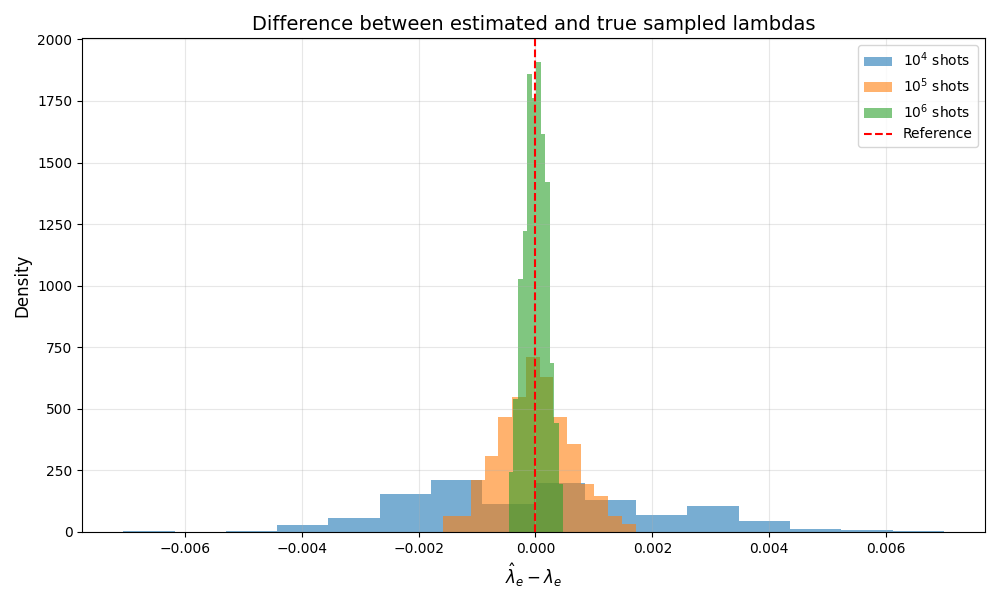
\includegraphics[width=\linewidth]{plot_lambda_diff_by_shots_sd_0002.png}
    %\caption{}
	%\caption{Distribution of the reconstruction differences for the 2D cluster-state with $12 \times 12$ simulation, shown for $10^4$, $10^5$, and $10^6$ shots. The dashed red line indicates zero difference. The distribution becomes increasingly concentrated around zero as the number of shots increases.}
	%\label{fig:lambda_diff_by_shots}
    \end{subfigure}
\hfill
\begin{subfigure}{0.48\textwidth}
	\centering
	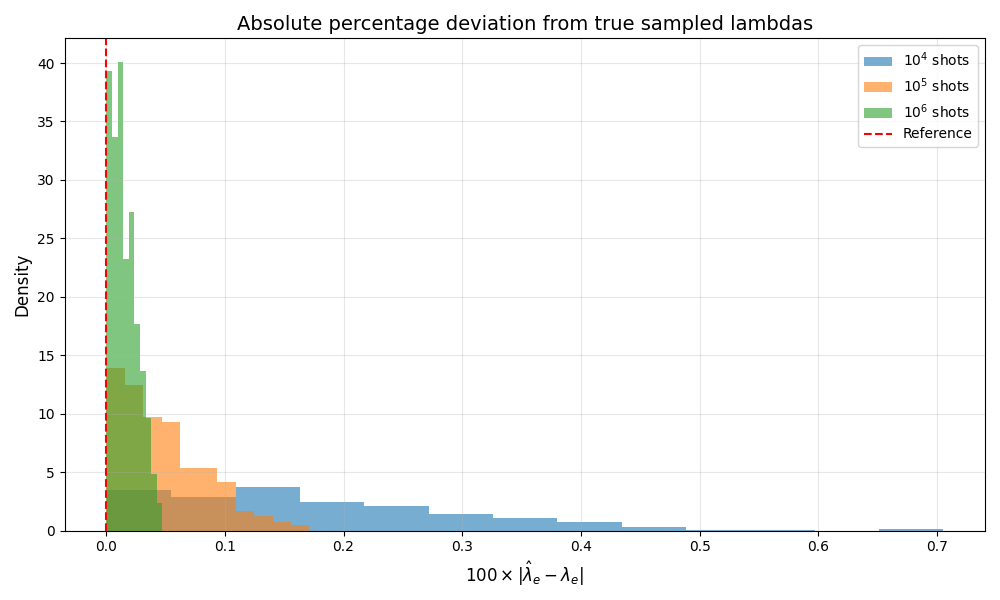
\includegraphics[width=\linewidth]{plot_lambda_diff_abs_by_shots_sd_0002.png}
    %\caption{}
	%\caption{Distribution of the absolute reconstruction deviations for the 2D cluster-state with $12 \times 12$ simulation, shown for $10^4$, $10^5$, and $10^6$ shots. The improved concentration near zero with increasing shot count indicates better reconstruction accuracy.}
	%\label{fig:lambda_abs_diff_by_shots}
\end{subfigure}
%%\vspace{-0.4cm}
\caption{Distribution of the reconstruction differences $\widehat{\lambda}_e-\lambda_e$
(left) and of the absolute deviations $100\times |\widehat{\lambda}_e-\lambda_e|$ (right)
for the $12\times 12$ 2D cluster-state, using $10^4$, $10^5$, and $10^6$ shots, when the
post-$\CZ$ one-qubit depolarizing error probabilities are sampled independently from
$\mathcal{N}(10^{-2},\,2\times 10^{-4})$. The dashed red line marks zero difference. The
reconstruction is centered near zero and becomes progressively more concentrated as the shot
count increases.}
 %   \caption{Distribution of the reconstruction differences for the 2D cluster-state with $12 \times 12$ simulation, shown for $10^4$, $10^5$, and $10^6$ shots. The dashed red line indicates zero difference. The distribution becomes increasingly concentrated around zero as the number of shots increases (left). Distribution of the absolute reconstruction deviations for the 2D cluster-state with $12 \times 12$ simulation, shown for $10^4$, $10^5$, and $10^6$ shots. The improved concentration near zero with increasing shot count indicates better reconstruction accuracy (right).}
    %\label{fig:placeholder}
\end{figure}
%%\hfill
%\vspace{-0.8cm}
    \begin{figure}[!h]
	\centering
    \begin{subfigure}{0.48\textwidth}
    %\centering
	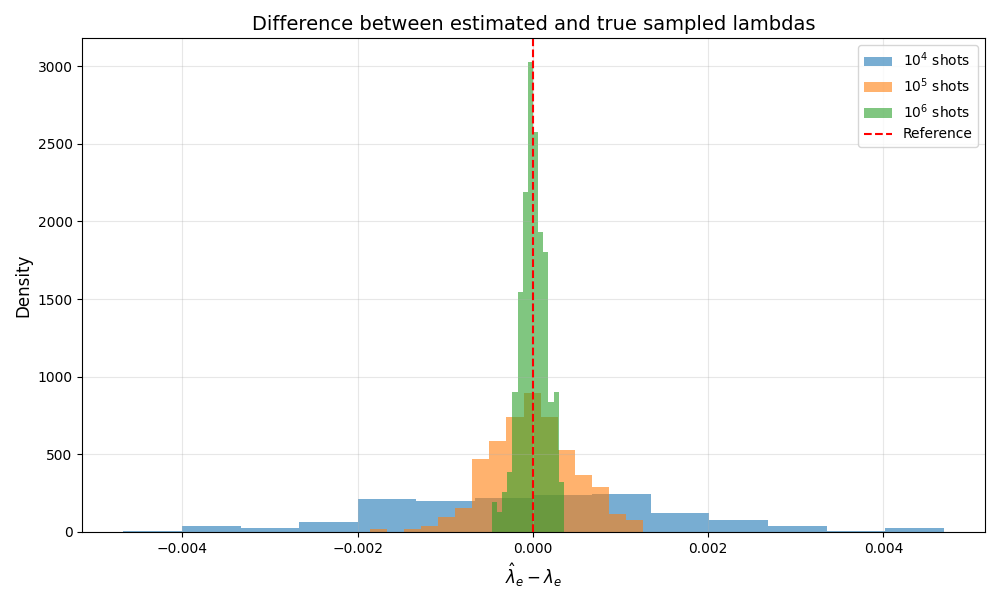
\includegraphics[width=\linewidth]{plot_lambda_diff_by_shots}
    %\caption{}
	%\caption{Distribution of the reconstruction differences for the 2D cluster-state with $12 \times 12$ simulation, shown for $10^4$, $10^5$, and $10^6$ shots. The dashed red line indicates zero difference. The distribution becomes increasingly concentrated around zero as the number of shots increases.}
	%\label{fig:lambda_diff_by_shots}
    \end{subfigure}
\hfill
\begin{subfigure}{0.48\textwidth}
	%\centering
	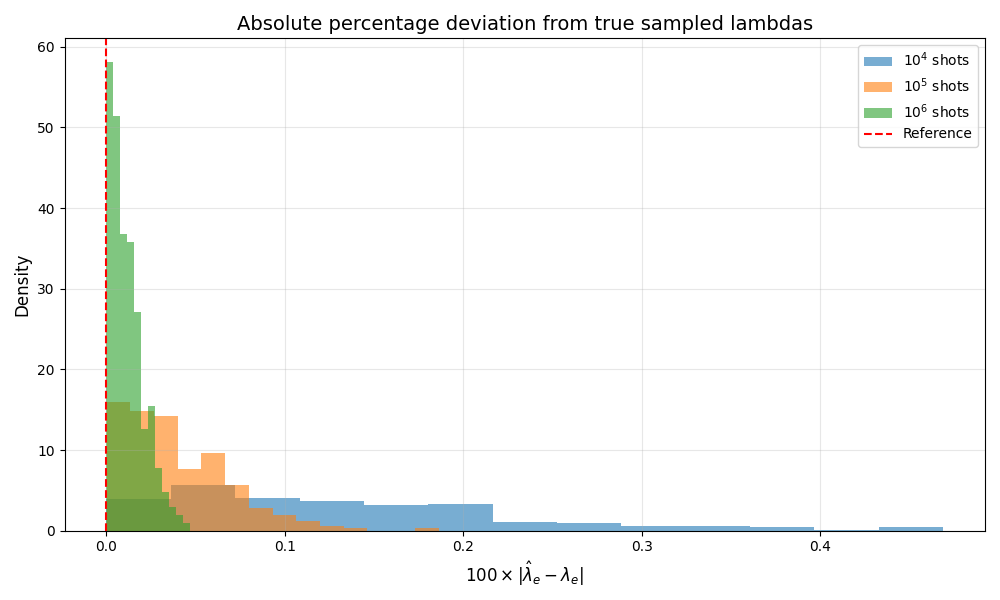
\includegraphics[width=\linewidth]{plot_lambda_diff_abs_by_shots}
    %\caption{}
	%\caption{Distribution of the absolute reconstruction deviations for the 2D cluster-state with $12 \times 12$ simulation, shown for $10^4$, $10^5$, and $10^6$ shots. The improved concentration near zero with increasing shot count indicates better reconstruction accuracy.}
	%\label{fig:lambda_abs_diff_by_shots}
\end{subfigure}
%\vspace{-0.4cm}
\caption{Distribution of the reconstruction differences $\widehat{\lambda}_e-\lambda_e$
(left) and of the absolute deviations $100\times |\widehat{\lambda}_e-\lambda_e|$ (right)
for the $12\times 12$ 2D cluster-state, using $10^4$, $10^5$, and $10^6$ shots, when the
post-$\CZ$ one-qubit depolarizing error probabilities are sampled independently from
$\mathcal{N}(10^{-2},\,2\times 10^{-5})$. The dashed red line marks zero difference. The
signed and absolute reconstruction errors both contract as more samples are collected.}
  %  \caption{Distribution of the reconstruction differences for the 2D cluster-state with $12 \times 12$ simulation, shown for $10^4$, $10^5$, and $10^6$ shots. The dashed red line indicates zero difference. The distribution becomes increasingly concentrated around zero as the number of shots increases (left). Distribution of the absolute reconstruction deviations for the 2D cluster-state with $12 \times 12$ simulation, shown for $10^4$, $10^5$, and $10^6$ shots. The improved concentration near zero with increasing shot count indicates better reconstruction accuracy (right).}
    %\label{fig:placeholder}
\end{figure}
%%\hfill
%\vspace{-0.4cm}
\begin{figure}[!h]
	\centering
    \begin{subfigure}{0.48\textwidth}
    %\centering
	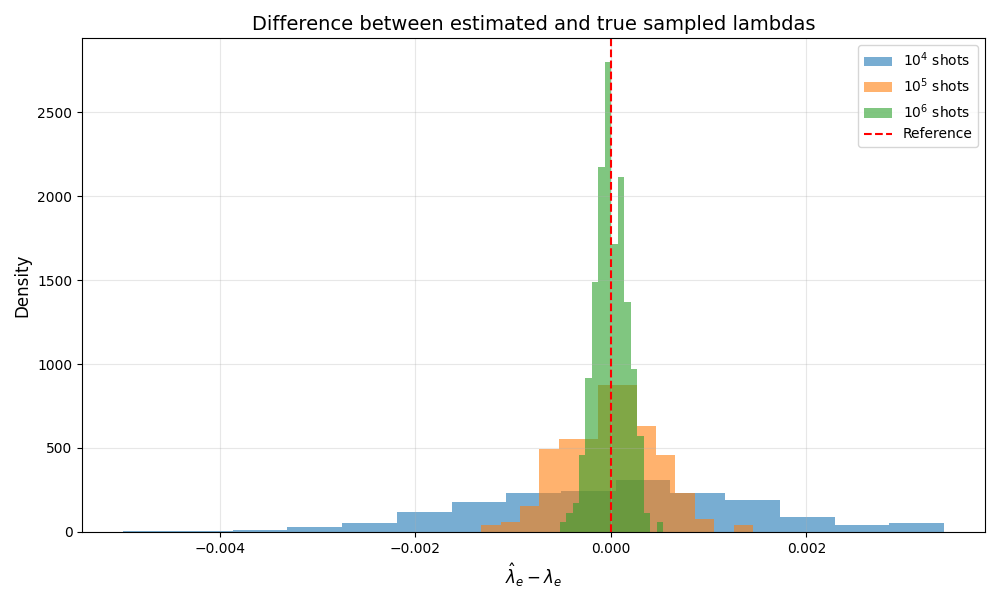
\includegraphics[width=\linewidth]{plot_lambda_diff_by_shots_sd_000002.png}
    %\caption{}
	%\caption{Distribution of the reconstruction differences for the 2D cluster-state with $12 \times 12$ simulation, shown for $10^4$, $10^5$, and $10^6$ shots. The dashed red line indicates zero difference. The distribution becomes increasingly concentrated around zero as the number of shots increases.}
	%\label{fig:lambda_diff_by_shots}
    \end{subfigure}
\hfill
\begin{subfigure}{0.48\textwidth}
	%\centering
	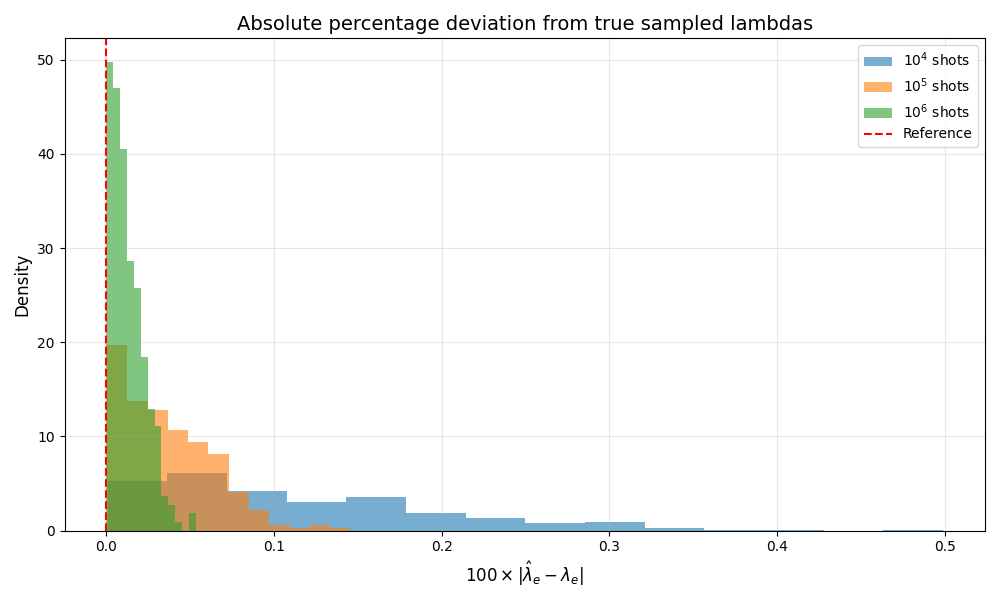
\includegraphics[width=\linewidth]{plot_lambda_diff_abs_by_shots_sd_000002.png}
    %\caption{}
	%\caption{Distribution of the absolute reconstruction deviations for the 2D cluster-state with $12 \times 12$ simulation, shown for $10^4$, $10^5$, and $10^6$ shots. The improved concentration near zero with increasing shot count indicates better reconstruction accuracy.}
	%\label{fig:lambda_abs_diff_by_shots}
\end{subfigure}
%\vspace{-0.4cm}
\caption{Distribution of the reconstruction differences $\widehat{\lambda}_e-\lambda_e$
(left) and of the absolute deviations $100\times |\widehat{\lambda}_e-\lambda_e|$ (right)
for the $12\times 12$ 2D cluster-state, using $10^4$, $10^5$, and $10^6$ shots, when the
post-$\CZ$ one-qubit depolarizing error probabilities are sampled independently from
$\mathcal{N}(10^{-2},\,2\times 10^{-6})$. The dashed red line marks zero difference. The
histograms remain centered near zero, while increasing the number of shots reduces the spread
of the reconstruction error.}
%    \caption{Distribution of the reconstruction differences for the 2D cluster-state with $12 \times 12$ simulation, shown for $10^4$, $10^5$, and $10^6$ shots. The dashed red line indicates zero difference. The distribution becomes increasingly concentrated around zero as the number of shots increases (left). Distribution of the absolute reconstruction deviations for the 2D cluster-state with $12 \times 12$ simulation, shown for $10^4$, $10^5$, and $10^6$ shots. The improved concentration near zero with increasing shot count indicates better reconstruction accuracy (right).}
    %\label{fig:placeholder}
\end{figure}
%%\hfill
%\vspace{-0.4cm}
\begin{figure}[!h]
	\centering
    \begin{subfigure}{0.48\textwidth}
    %\centering
	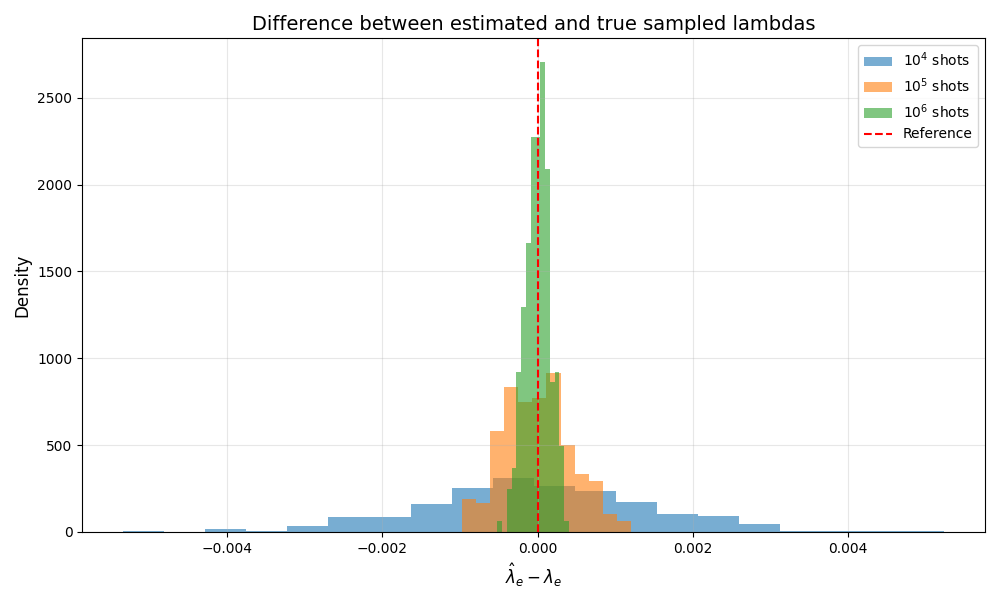
\includegraphics[width=\linewidth]{plot_lambda_diff_by_shots_sd_0000002.png}
    %\caption{}
	%\caption{Distribution of the reconstruction differences for the 2D cluster-state with $12 \times 12$ simulation, shown for $10^4$, $10^5$, and $10^6$ shots. The dashed red line indicates zero difference. The distribution becomes increasingly concentrated around zero as the number of shots increases.}
	%\label{fig:lambda_diff_by_shots}
    \end{subfigure}
\hfill
\begin{subfigure}{0.48\textwidth}
	%\centering
	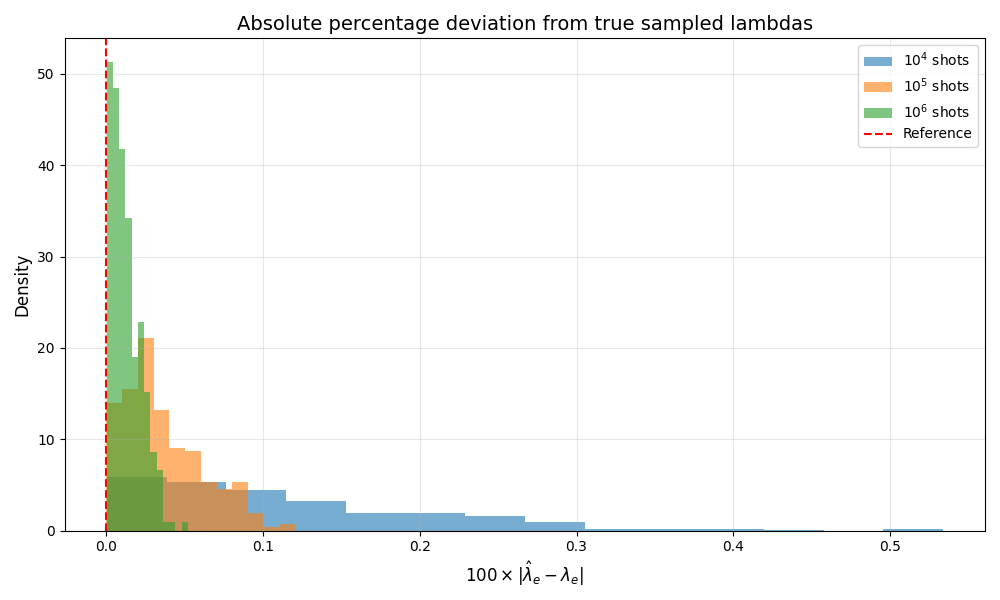
\includegraphics[width=\linewidth]{plot_lambda_diff_abs_by_shots_sd_0000002.png}
    %\caption{}
	%\caption{Distribution of the absolute reconstruction deviations for the 2D cluster-state with $12 \times 12$ simulation, shown for $10^4$, $10^5$, and $10^6$ shots. The improved concentration near zero with increasing shot count indicates better reconstruction accuracy.}
	%\label{fig:lambda_abs_diff_by_shots}
\end{subfigure}
%\vspace{-0.4cm}
\caption{Distribution of the reconstruction differences $\widehat{\lambda}_e-\lambda_e$
(left) and of the absolute deviations $100\times |\widehat{\lambda}_e-\lambda_e|$ (right)
for the $12\times 12$ 2D cluster-state, using $10^4$, $10^5$, and $10^6$ shots, when the
post-$\CZ$ one-qubit depolarizing error probabilities are sampled independently from
$\mathcal{N}(10^{-2},\,2\times 10^{-7})$. The dashed red line marks zero difference. This is
the most concentrated noise ensemble among the five cases, and the reconstruction errors shrink
further as the shot count increases.}
%\caption{Distribution of the reconstruction differences for the 2D cluster-state with $12 \times 12$ simulation, shown for $10^4$, $10^5$, and $10^6$ shots. The dashed red line indicates zero difference. The distribution becomes increasingly concentrated around zero as the number of shots increases (left). Distribution of the absolute reconstruction deviations for the 2D cluster-state with $12 \times 12$ simulation, shown for $10^4$, $10^5$, and $10^6$ shots. The improved concentration near zero with increasing shot count indicates better reconstruction accuracy (right).}
\label{fig:lambda_abs_diff_by_shots}
\end{figure}



